\section{Power Circuit Block diagram}

To design the power circuit for the flexible voice coil actuator, we started by analyzing the requirements of the actuator.
First of all, we want the coil to be driven with a sinusoidal \textbf{AC signal} at various frequencies and amplitudes; so the first component to consider it's the \textbf{system's controller} which in this case, can be a \textbf{simple signal generator}.
For our application, we chose a simple \textbf{ESP32} microcontroller, which has an \textbf{integrated DAC}.
\bigskip

Then we have to consider the \textbf{power requirements} to run the chosen coil.
The impedance of a Flexar coil, as we discussed before, is in the order of 30$\Omega$.
The impedance of the coil is \textbf{too low} to be driven directly by the ESP32 DAC, so a \textbf{power stage} is needed.
For the sake of simplicity, we chose to implement a power stage with a \textbf{fixed gain} of 10.
\bigskip

Then we want the amplitude of the signal to be adjustable, so we needed a \textbf{conditioning circuit} to adjust the amplitude of the signal coming from the DAC \textbf{before being amplified}.
\bigskip

The control circuit can be summarized as a block diagram, as shown in figure \ref{fig: Power_Circuit_Block_Diagram}.
\begin{figure}[H]
    \centering
    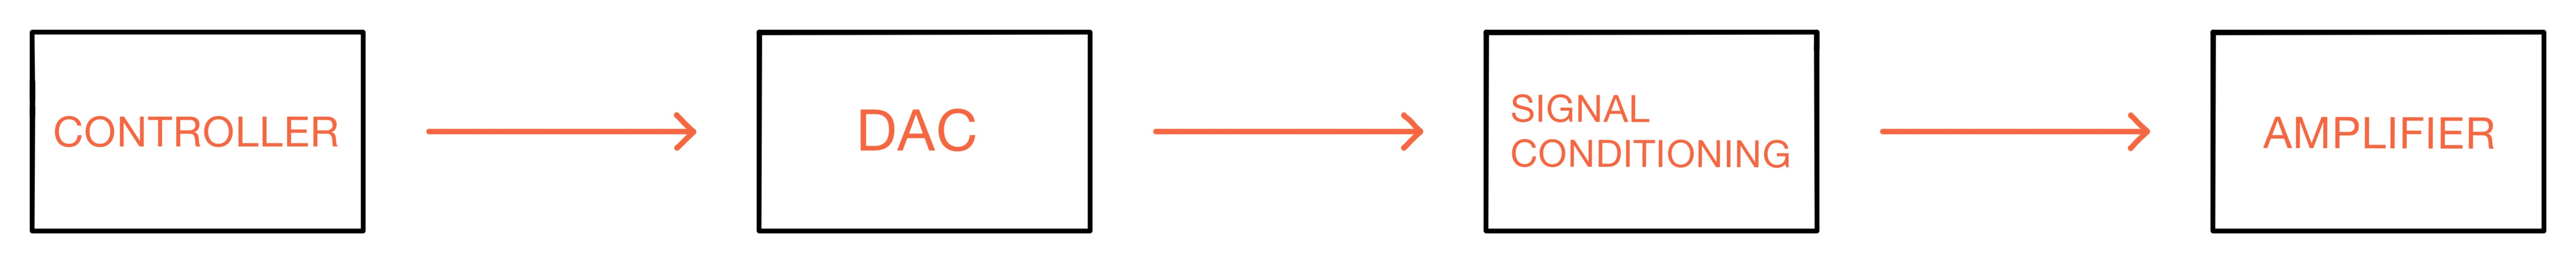
\includegraphics[width=1\linewidth]{Chapters/Chapter4/Figures/power_circuit_block_diagram.jpg}
    \caption{Block diagram of the power circuit.}
    \label{fig: Power_Circuit_Block_Diagram}    
\end{figure}

\pagebreak